\documentclass{standalone}
\usepackage{tikz,pgfplots,calc}
\usetikzlibrary{positioning,calc}
\usetikzlibrary{arrows}
\usepackage{tkz-euclide}
\usetkzobj{all}

\tikzset{
  mynode/.style = {align = center}}

\begin{document}
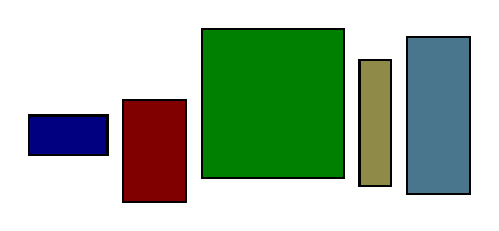
\begin{tikzpicture}[>=stealth', thick]

\draw [draw, fill = blue!50!black] (0, 0.5) rectangle (1, 1);
\draw [draw, fill = red!50!black] (1.2, -.1) rectangle (2, 1.2);
\draw [draw, fill = green!50!black] (2.2, .2) rectangle (4, 2.1);
\draw [draw, fill = yellow!50!black] (4.2, .1) rectangle (4.6, 1.7);
\draw [draw, fill = cyan!50!black] (4.8, 0) rectangle (5.6, 2.);
\end{tikzpicture}
\end{document}